\documentclass{oblivoir}
\usepackage{amsmath,amssymb,amsthm,kotex,paralist,kswrapfig,graphicx}

\usepackage[skipabove=10pt,skipbelow=10pt]{mdframed}
\setlength\intextsep{0pt}

\usepackage{tabto,pifont}
\TabPositions{0.2\textwidth,0.4\textwidth,0.6\textwidth,0.8\textwidth}
\newcommand\tabb[5]{\par\bigskip\noindent
\ding{172}\:{\ensuremath{#1}}
\tab\ding{173}\:\:{\ensuremath{#2}}
\tab\ding{174}\:\:{\ensuremath{#3}}
\tab\ding{175}\:\:{\ensuremath{#4}}
\tab\ding{176}\:\:{\ensuremath{#5}}}

\usepackage{enumitem}
\setlist[enumerate]{label=(\arabic*)}

\newcounter{num}
\newcommand{\defi}[1]
{\bigskip\noindent\refstepcounter{num}\textbf{정의 \arabic{num}) #1}\par\noindent}
\newcommand{\theo}[1]
{\bigskip\noindent\refstepcounter{num}\textbf{정리 \arabic{num}) #1}\par\noindent}
\newcommand{\exam}[1]
{\bigskip\noindent\refstepcounter{num}\textbf{예시 \arabic{num}) #1}\par\noindent}
\newcommand{\prob}[1]
{\bigskip\noindent\refstepcounter{num}\textbf{문제 \arabic{num}) #1}\par\noindent}
\newcommand{\proo}
{\bigskip\textsf{증명)}\par}

\newcommand{\ans}{
{\par
\raggedleft\textbf{답 : (\qquad\qquad\qquad\qquad\qquad\qquad)}
\par}\bigskip\bigskip}
\newcommand\an[1]{\par\bigskip\noindent\textbf{문제 #1)}\\}

\newcommand{\pb}[1]%\Phantom + fBox
{\fbox{\phantom{\ensuremath{#1}}}}

\newcommand{\procedure}[1]{\begin{mdframed}\vspace{#1\textheight}\end{mdframed}}
\newcommand\ba{\,|\,}

\let\oldsection\section
\let\emph\textsf
\renewcommand\section{\clearpage\oldsection}
%%%%
\begin{document}

\title{미적분 1 : 03 함수의 극한}
\author{}
\date{\today}
\maketitle
\tableofcontents
\newpage

%%
\section{함수의 극한}

\begin{mdframed}[innertopmargin=-5pt]
%
\kswrapfig[Pos=r,Width=3cm]{constant_converge}{
\setcounter{num}0
\defi{\(x\to a\)일 때의 함수의 수렴}
함수 \(f(x)\)에서 \(x\)의 값이 \(x\neq a\)을 만족시키면서 한없이 \(a\)에 가까워질 때, \(f(x)\)의 값이 일정한 값 \(L\)에 한없이 가까워지면 
\medskip
\begin{center}
\(x\)가 \(a\)에 가까워질 때, \(f(x)\)는 \(L\)에 \emph{수렴}한다.
\end{center}
\medskip\par
\noindent라고 말하고 기호로
\[\lim_{x\to a}f(x)=L\]
로 나타낸다.
이때 \(L\)을 \(f(x)\)의 \emph{극한값}이라고 부른다.}
\end{mdframed}

%
\exam{}
\(f(x)=x+2\)이면 함수의 그래프는 아래 왼쪽 그림과 같다.
따라서 \(x\)가 \(1\)에 한없이 가까워질수록 \(f(x)\)는 \(3\)에 가까워진다.
\[\lim_{x\to1}(x+2)=3\]
\begin{figure*}[h!]
\noindent\centering
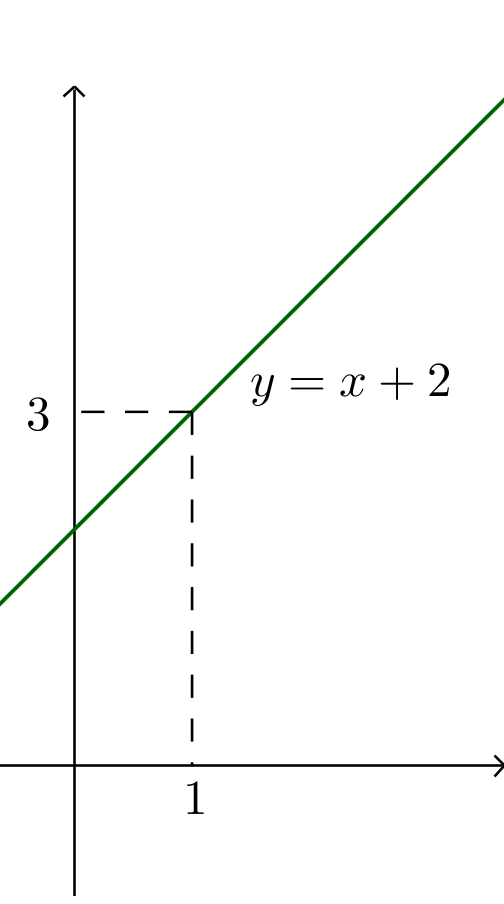
\includegraphics[width=0.3\textwidth]{y=x+2}
\hspace{10pt}
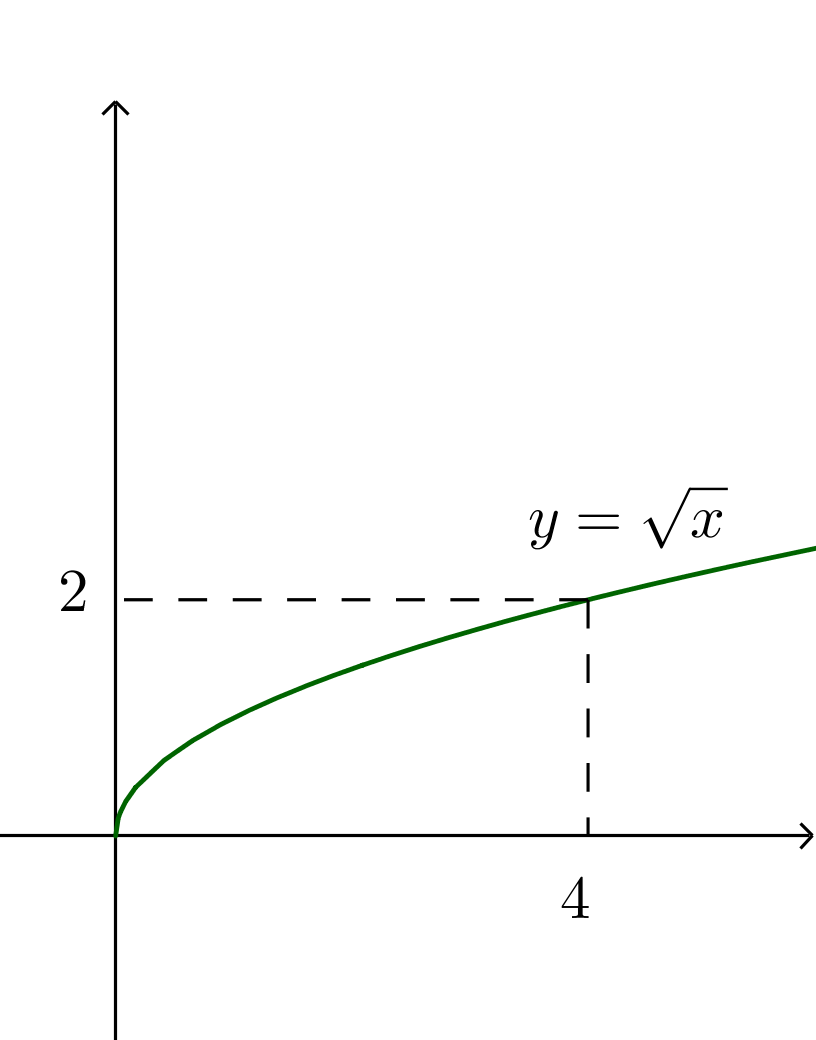
\includegraphics[width=0.4\textwidth]{y=sqrtx}
\end{figure*}


\clearpage
%
\exam{}
\(f(x)=\sqrt x\)이면 함수의 그래프는 위의 오른쪽 그림과 같다.
따라서
\(x\)가 \(4\)에 한없이 가까워질수록 \(f(x)\)는 \(2\)에 가까워진다.
\[\lim_{x\to4}\sqrt x=2\]

\kswrapfig[Pos=r,Width=3cm]{y=x+2_2}{
%
%\setcounter{num}3
\exam{}
\(f(x)=\frac{x^2+x-2}{x-1}\)이면, %\(f\)의 정의역은 \(\{x\ba x\neq1\}\)이고,
\(x\neq1\)일 때
\[f(x)=\frac{(x-1)(x+2)}{x-1}=x+2%\qquad(x\neq1)
\]
이다.
따라서  함수의 그래프는 오른쪽 그림과 같다.
이때, 함숫값 \(f(1)\)은 존재하지 않지만 극한값
\[\lim_{x\to1}\frac{x^2+x-2}{x-1}=3\]
은 존재한다.
}

%
\prob{}
\noindent(1)\:\:
\(y=\frac4x\)의 그래프를 그리고, \(\displaystyle\lim_{x\to2}\:\frac4x\:\)를 구하여라.
\begin{figure*}[h!]
\centering
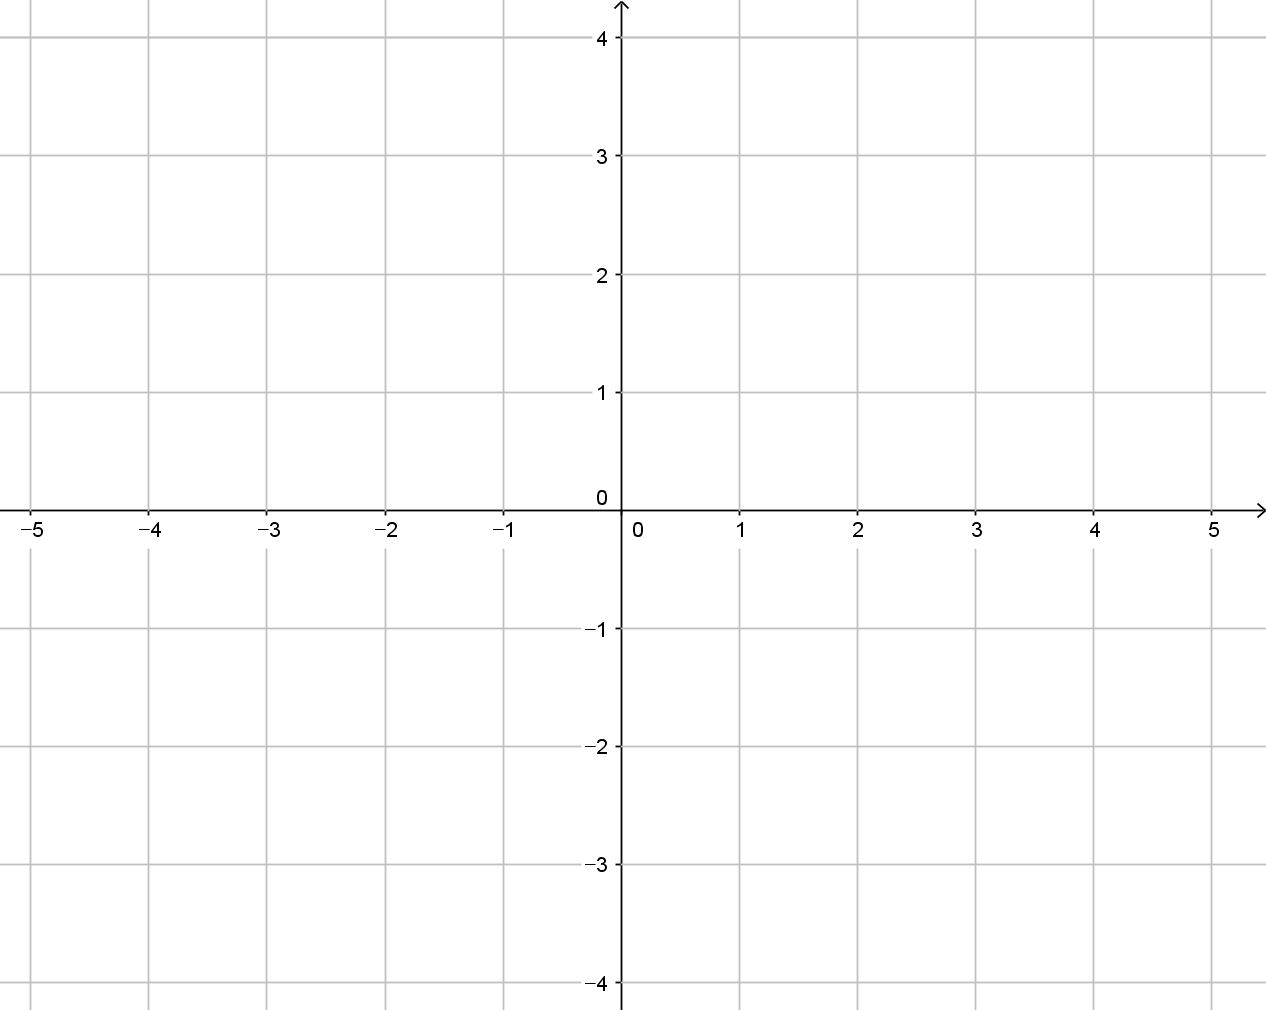
\includegraphics[width=0.6\textwidth]{5times4}
\end{figure*}
\begin{flushright}
\textbf{답 : }\(\displaystyle\lim_{x\to2}\:\frac4x\:=\pb1.\)
\end{flushright}

\clearpage
\noindent(2)\:\:
\(y=\frac{x^2+2x}x\)의 그래프를 그리고, \(\displaystyle\lim_{x\to0}\frac{x^2+2x}x\)를 구하여라.
\begin{figure*}[h!]
\centering
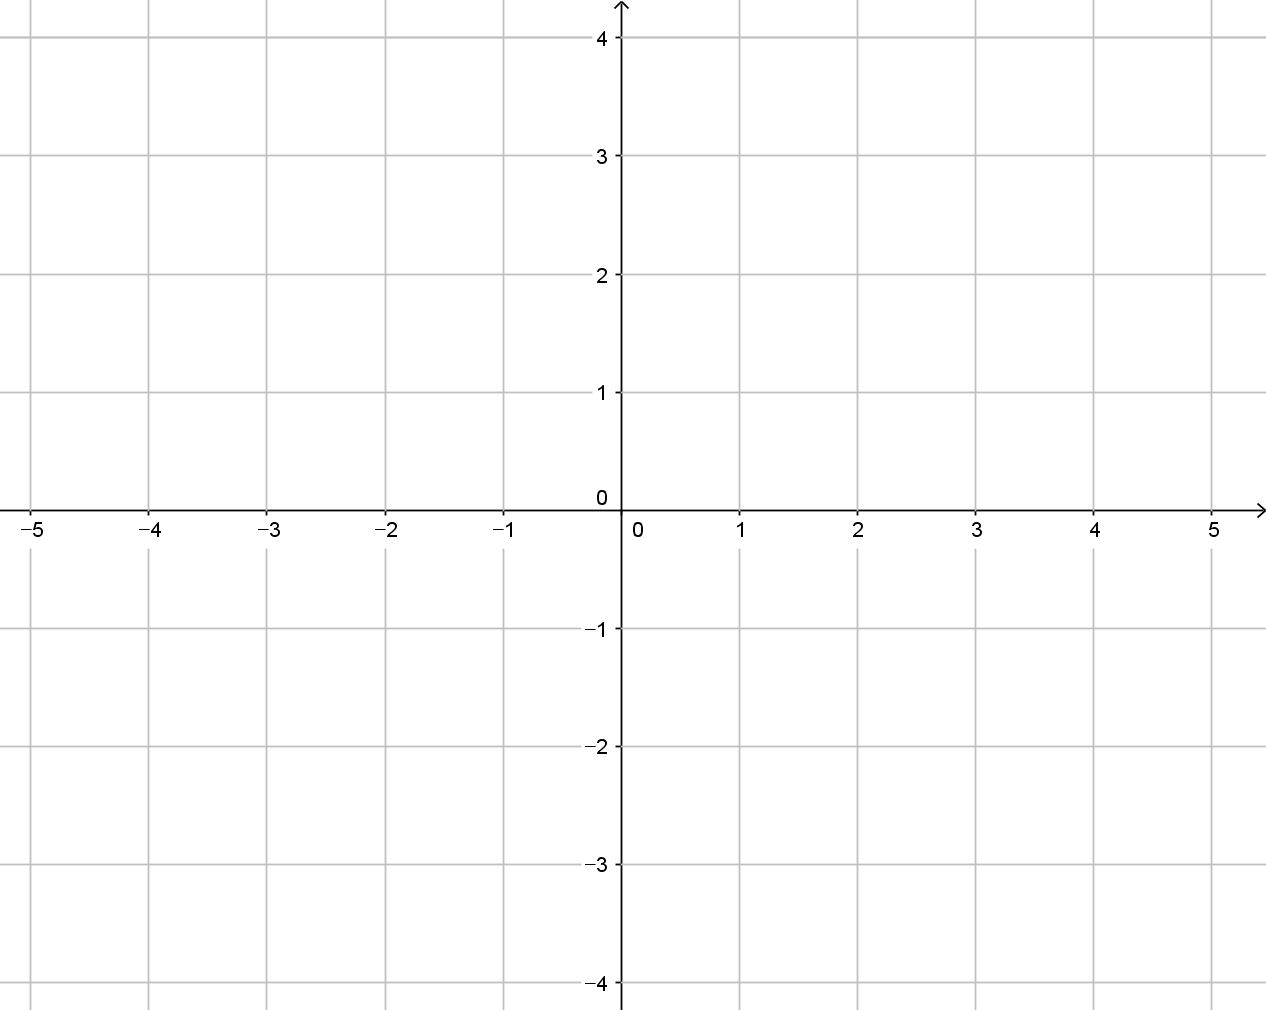
\includegraphics[width=0.6\textwidth]{5times4}
\end{figure*}
\begin{flushright}
\textbf{답 : }\(\displaystyle\lim_{x\to0}\frac{x^2+2x}x=\pb1.\)
\end{flushright}

\vspace{0.1\textheight}
\noindent(3)\:\:
\(y=\frac{x^3-5x^2+4x}{x-1}\)의 그래프를 그리고, \(\displaystyle\lim_{x\to1}\frac{x^3-5x^2+4x}{x-1}\)를 구하여라.
\begin{figure*}[h!]
\centering
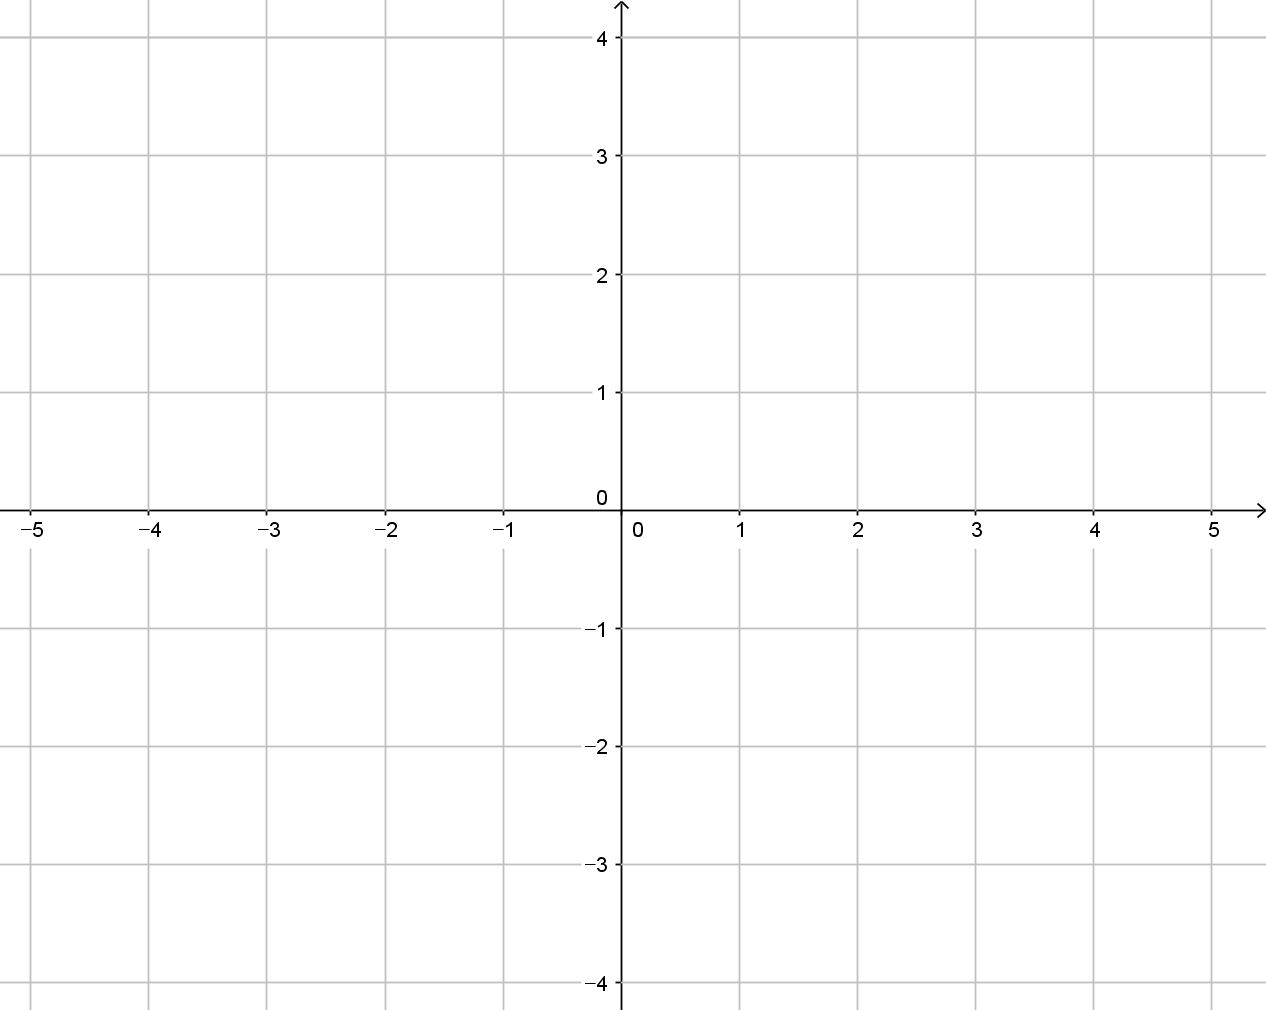
\includegraphics[width=0.6\textwidth]{5times4}
\end{figure*}
\begin{flushright}
\textbf{답 : }\(\displaystyle\lim_{x\to1}\frac{x^3-5x^2+4x}{x-1}=\pb1.\)
\end{flushright}

\clearpage
\begin{mdframed}[innertopmargin=-5pt]
%
\kswrapfig[Pos=r,Width=3cm]{infty_converge}{
\setcounter{num}5
\defi{\(x\to\pm\infty\)일 때의 함수의 수렴}
함수 \(f(x)\)에서 \(x\)의 값이 한없이 커질 때, \(f(x)\)의 값이 일정한 값 \(L\)에 한없이 가까워지면
\[\lim_{x\to \infty}f(x)=L\]
로 나타낸다.
또, \(x\)의 값이 한없이 작아질 때, \(f(x)\)의 값이 일정한 값 \(M\)에 한없이 가까워지면 
\[\lim_{x\to-\infty}f(x)=M\]
로 나타낸다.}
\end{mdframed}

\kswrapfig[Pos=r,Width=3cm]{y=frac1x}{
\vspace{-15pt}
%
\setcounter{num}6
\exam{}
\(f(x)=\frac1x\)이면 함수의 그래프는 아래 그림과 같다.
따라서
\[\lim_{x\to\infty}\frac1x=0\]
\[\lim_{x\to-\infty}\frac1x=0\]
}

\vspace{-20pt}
%
\prob{}
\(y=\frac x{x-1}\)의 그래프를 그리고, \(\displaystyle\lim_{x\to\infty}\frac x{x-1}\)와 \(\displaystyle\lim_{x\to-\infty}\frac x{x-1}\)를 구하여라.
\begin{figure*}[h!]
\centering
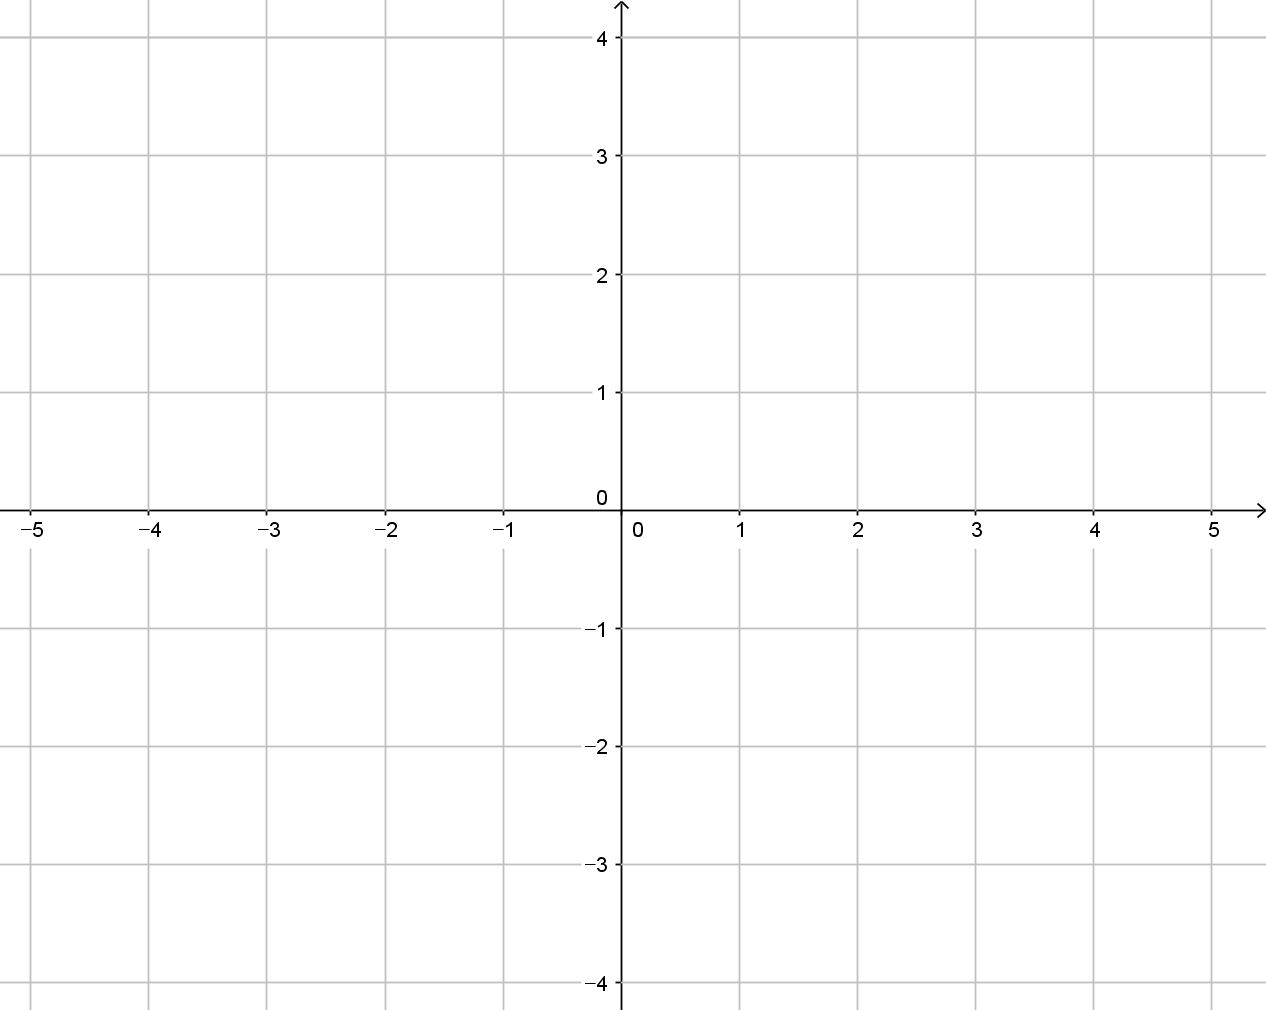
\includegraphics[width=0.6\textwidth]{5times4}
\end{figure*}
\begin{flushright}
\textbf{답 : }\(\displaystyle\lim_{x\to\infty}\frac x{x-1}=\pb1\),\qquad\(\displaystyle\lim_{x\to-\infty}\frac x{x-1}=\pb1.\)
\end{flushright}

%\kswrapfig[Pos=r,Width=3cm]{xyaxis}{
%\(f(x)=\frac{3x-1}{x-1}\)이면 함수의 그래프는 오른쪽 그림과 같고, \(x\)가 한없이 커질 때, \(f(x)\)의 값은 \(\pb3\)에 한없이 가까워진다.
%따라서
%\[\lim_{x\to\infty}\frac{3x-1}{x-1}=\pb3\]
%또, \(x\)의 값이 한없이 작아져도, \(f(x)\)의 값은 \(\pb3\)에 한없이 가까워진다.
%따라서
%\[\lim_{x\to-\infty}\frac{3x-1}{x-1}=\pb3\]
%}

\begin{mdframed}[innertopmargin=-5pt]
%
\kswrapfig[Pos=r,Width=3cm]{constant_diverge}{
\setcounter{num}{8}
\defi{\(x\to a\)일 때의 함수의 발산}
함수 \(f(x)\)에서 \(x\)의 값이 \(x\neq a\)을 만족시키면서 한없이 \(a\)에 가까워질 때, \(f(x)\)의 값이 한없이 커지면
\[\lim_{x\to a}f(x)=\infty\]
로 나타낸다.
또 \(x\)의 값이 한없이 \(a\)에 가까워질 때, \(f(x)\)의 값이 한없이 작아지면
\[\lim_{x\to a}f(x)=-\infty\]
로 나타낸다.}
\end{mdframed}

%
\prob{}
\(y=\frac1{x^2}\)의 그래프를 그리고, \(\displaystyle\lim_{x\to0}\frac1{x^2}\)를 구하여라.
\begin{figure*}[h!]
\centering
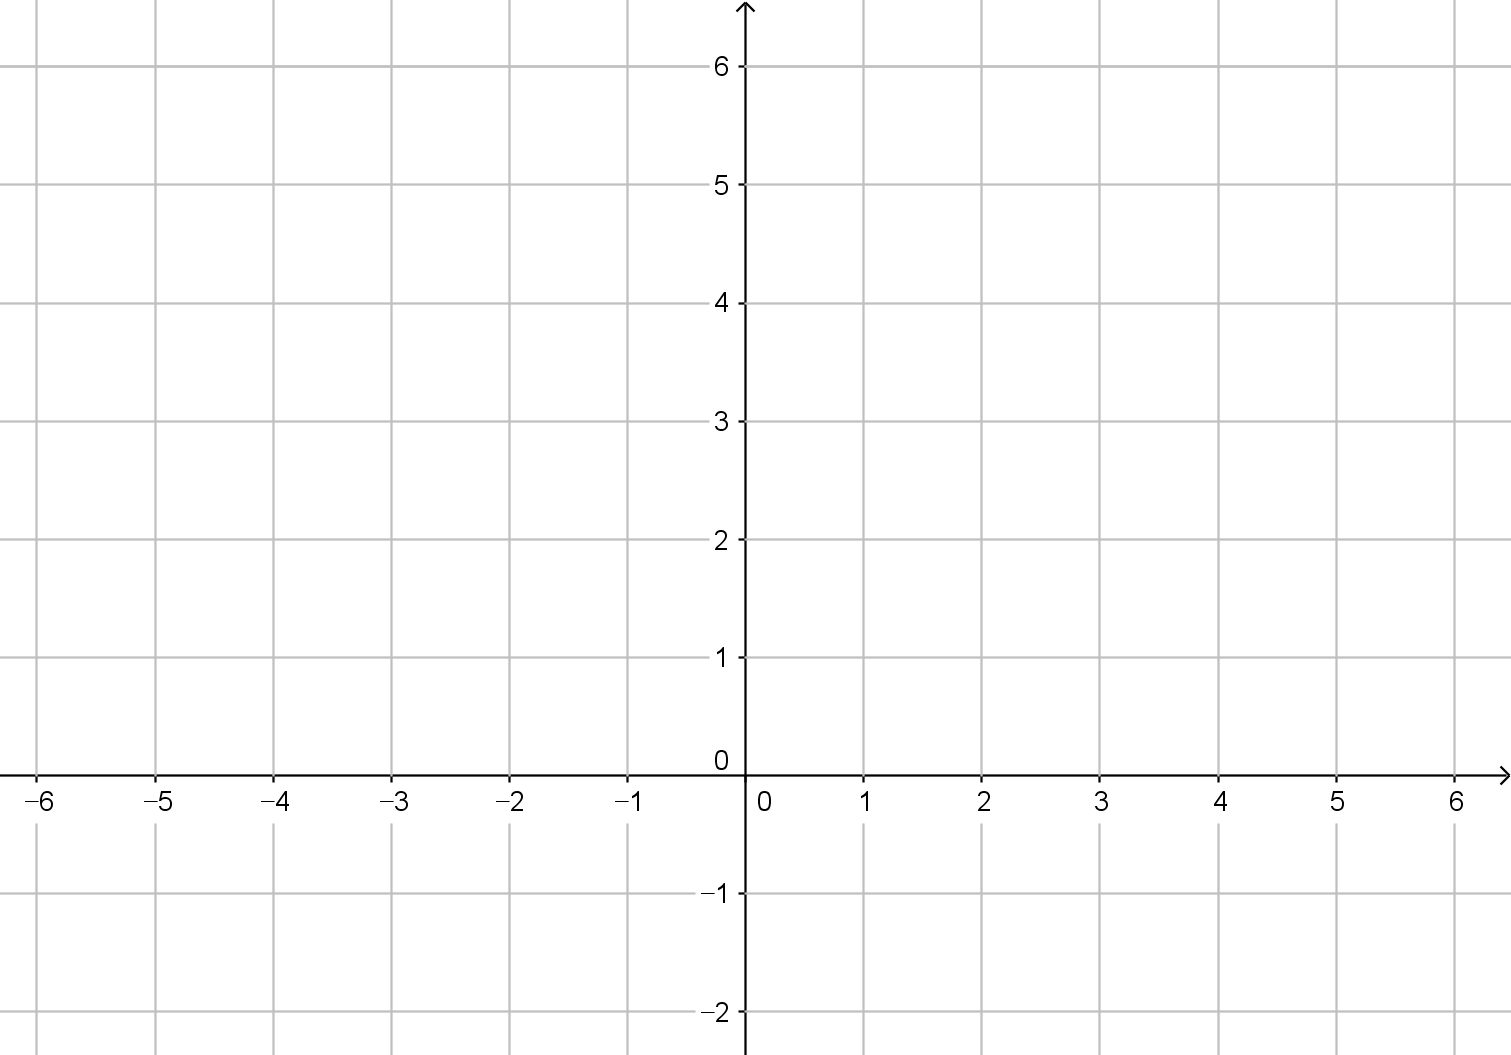
\includegraphics[width=0.6\textwidth]{6times6}
\end{figure*}
\begin{flushright}
\textbf{답 : }\(\displaystyle\lim_{x\to0}\frac1{x^2}=\pb1.\)
\end{flushright}
\clearpage

\begin{mdframed}[innertopmargin=-5pt]
%
\defi{\(x\to\pm\infty\)일 때의 함수의 발산}
함수 \(f(x)\)에서 \(x\)의 값이 한없이 커지거나 작아질 때, \(f(x)\)의 값이 한없이 커지거나 작아지면 다음과 같이 나타낸다.
\begin{gather*}
\lim_{x\to\infty}f(x)=\infty,\\
\lim_{x\to\infty}f(x)=-\infty,\\
\lim_{x\to-\infty}f(x)=\infty,\\
\lim_{x\to-\infty}f(x)=-\infty
\end{gather*}
\end{mdframed}

%
\prob{}
\(y=-\frac12x+1\)의 그래프를 그리고, \(\displaystyle\lim_{x\to\infty}\left(-\frac12x+1\right)\)와 \(\displaystyle\lim_{x\to-\infty}\left(-\frac12x+1\right)\)를 구하여라.
\begin{figure*}[h!]
\centering
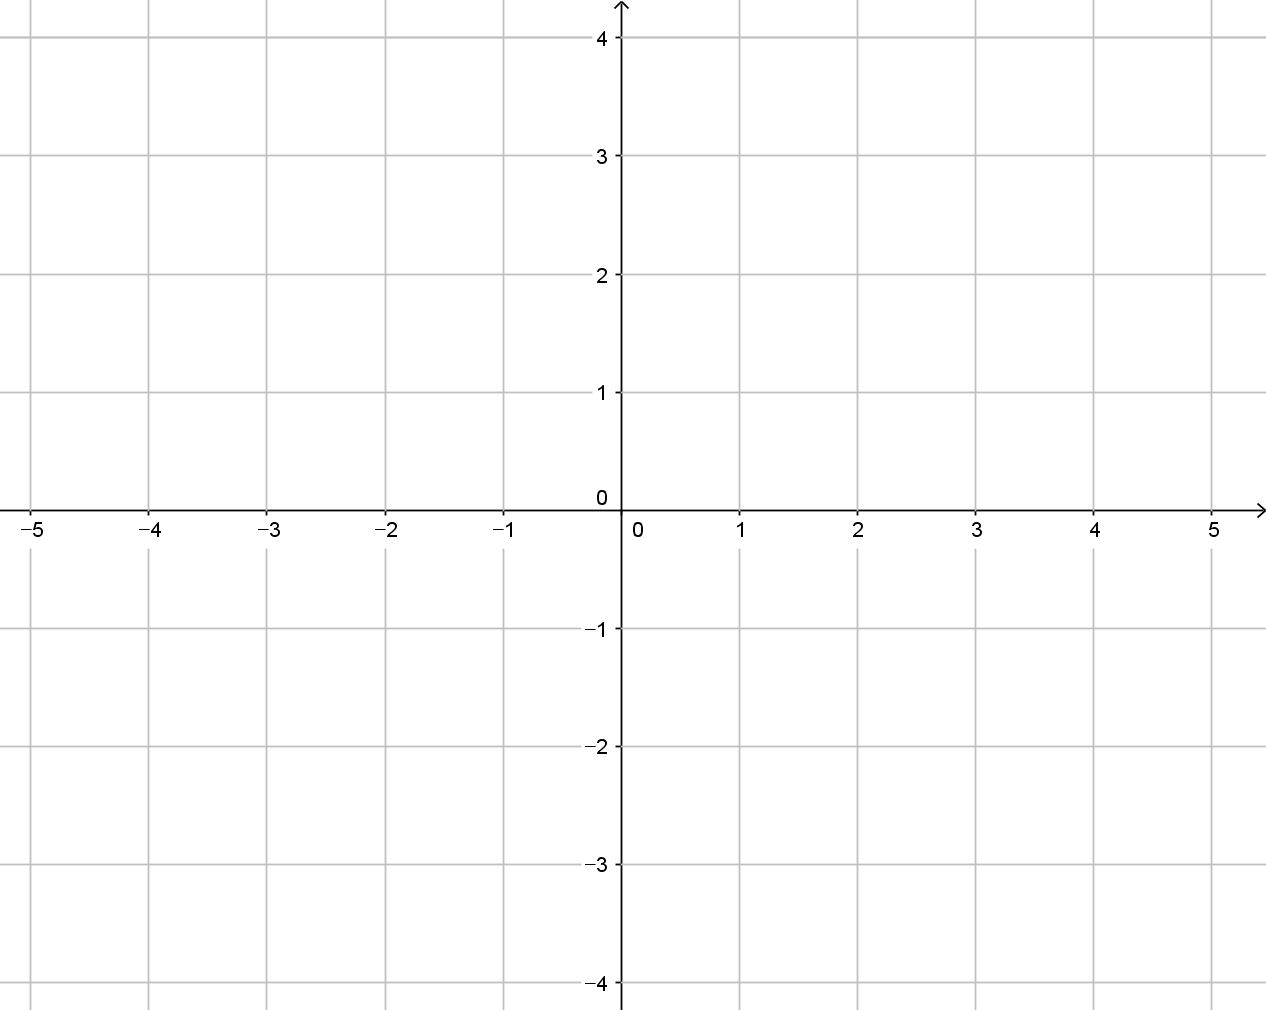
\includegraphics[width=0.6\textwidth]{5times4}
\end{figure*}
\begin{flushright}
\textbf{답 : }\(\displaystyle\lim_{x\to\infty}\left(-\frac12x+1\right)=\pb1\),\qquad\(\displaystyle\lim_{x\to-\infty}\left(-\frac12x+1\right)=\pb1.\)
\end{flushright}

%
\prob{}
\begin{enumerate}
\item
\(\displaystyle\lim_{x\to\infty}x^2=\)
\item
\(\displaystyle\lim_{x\to-\infty}x^2=\)
\end{enumerate}

\section{좌극한과 우극한}

\begin{mdframed}[innertopmargin=-5pt]
%
\kswrapfig[Pos=r,Width=3cm]{casewise_0}{
\setcounter{num}{13}
\defi{좌극한과 우극한}
함수 \(f(x)\)에서 \(x\)의 값이 \(x<a\)를 만족시키면서 한없이 \(a\)에 가까워질 때, \(f(x)\)의 값이 일정한 값 \(L\)에 한없이 가까워지면 
\[\lim_{x\to a-}f(x)=L\]
로 나타낸다.
또, \(x\)의 값이 \(x>a\)를 만족시키면서 한없이 \(a\)에 가까워질 때, \(f(x)\)의 값이 일정한 값 \(L\)에 가까워지면
\[\lim_{x\to a+}f(x)=M\]
이때 \(L\)과 \(M\)을 각각 \emph{좌극한}, \emph{우극한}이라고 부른다.}
\end{mdframed}

%
\exam{}\label{discontinuous}
\kswrapfig[Pos=r,Width=4cm]{casewise_1}{
함수 \(f(x)\)가
\[f(x)=
\begin{cases}
-x+2	&(x<1)\\
x+1	&(x\ge1)
\end{cases}\]
와 같이 주어지면 함수의 그래프는 오른쪽 그림과 같다.
이때,
\begin{gather*}
\lim_{x\to1-}f(x)=1\\
\lim_{x\to1+}f(x)=2
\end{gather*}
이다.}

\clearpage

%
\exam{}\label{continuous}
\kswrapfig[Pos=r,Width=3cm]{y=x+2_g}{
\noindent
\(g(x)=x+2\)이면 함수의 그래프는 오른쪽 그림과 같다.
이때,
\begin{gather*}
\lim_{x\to1-}g(x)=3\\
\lim_{x\to1+}g(x)=3
\end{gather*}
이다.}

예시 \ref{discontinuous}의 경우 함수 \(f(x)\)는
\[
\lim_{x\to1-}f(x)=1,\quad
\lim_{x\to1+}f(x)=2
\]
이다.
한편, \(\displaystyle\lim_{x\to1}f(x)\)
는 존재하지 않는다.

예시 \ref{continuous}의 경우 함수 \(g(x)\)는
\[\lim_{x\to1-}g(x)=3,\quad
\lim_{x\to1+}g(x)=3\]
이다.
또한
\(\displaystyle\lim_{x\to1}g(x)=3\)
이다.

\begin{mdframed}[innertopmargin=-5pt]
%
\theo{극한값이 존재하기 위한 조건}
함수 \(f(x)\)의 \(x=a\)에서의 극한값 \(\displaystyle\lim_{x\to a}f(x)\)가 존재하기 위한 조건은
\[\lim_{x\to a-}f(x)=\lim_{x\to a+}f(x)\]
이다.
\end{mdframed}

\clearpage
%
\prob{}
다음 함수들의 그래프를 그리고 주어진 점\(\langle x=a\rangle\)에서의 좌극한값, 우극한값, 극한값을 각각 구하여라.
(극한값이 존재하지 않는 경우 \(\times\)로 표시하시오.)
\begin{enumerate}
%
\item
\(f(x)=\sqrt x\), \tabto{0.5\textwidth}\(\langle x=4\rangle\)
\begin{figure*}[h!]
\centering
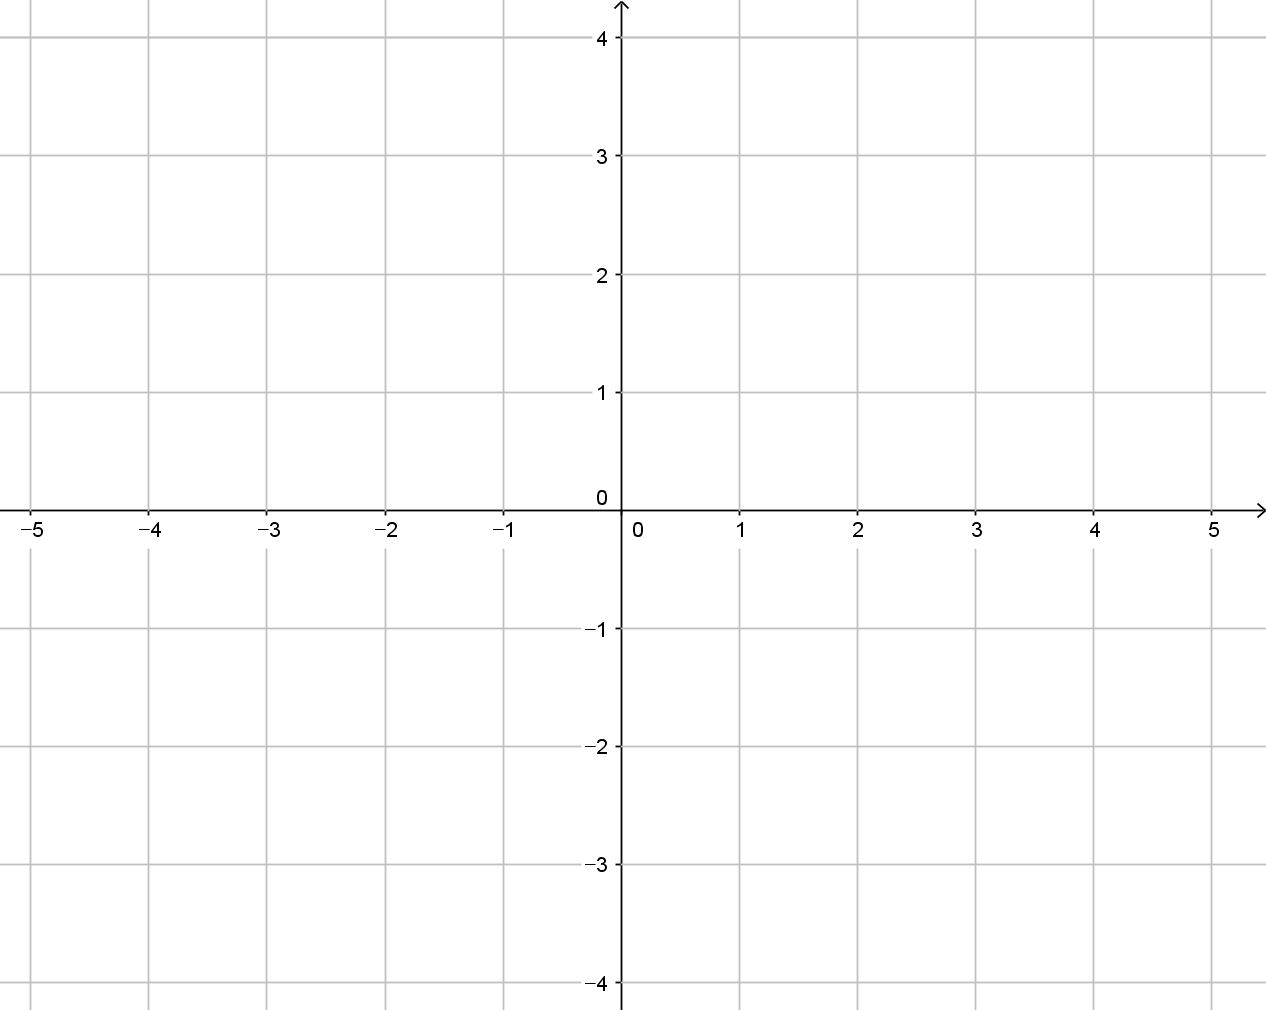
\includegraphics[width=0.5\textwidth]{5times4}
\end{figure*}\\
\[
\textbf{답 : }
\lim_{x\to4-}f(x)=\pb1,\qquad
\lim_{x\to4+}f(x)=\pb1,\qquad
\lim_{x\to4}f(x)=\pb1.
\]
%
\item
\(g(x)=
\begin{cases}
-x-3	&(x<-2)\\
2	&(x\ge-2)
\end{cases}\)
\tabto{0.5\textwidth}\(\langle x=-2\rangle\)
\begin{figure*}[h!]
\centering
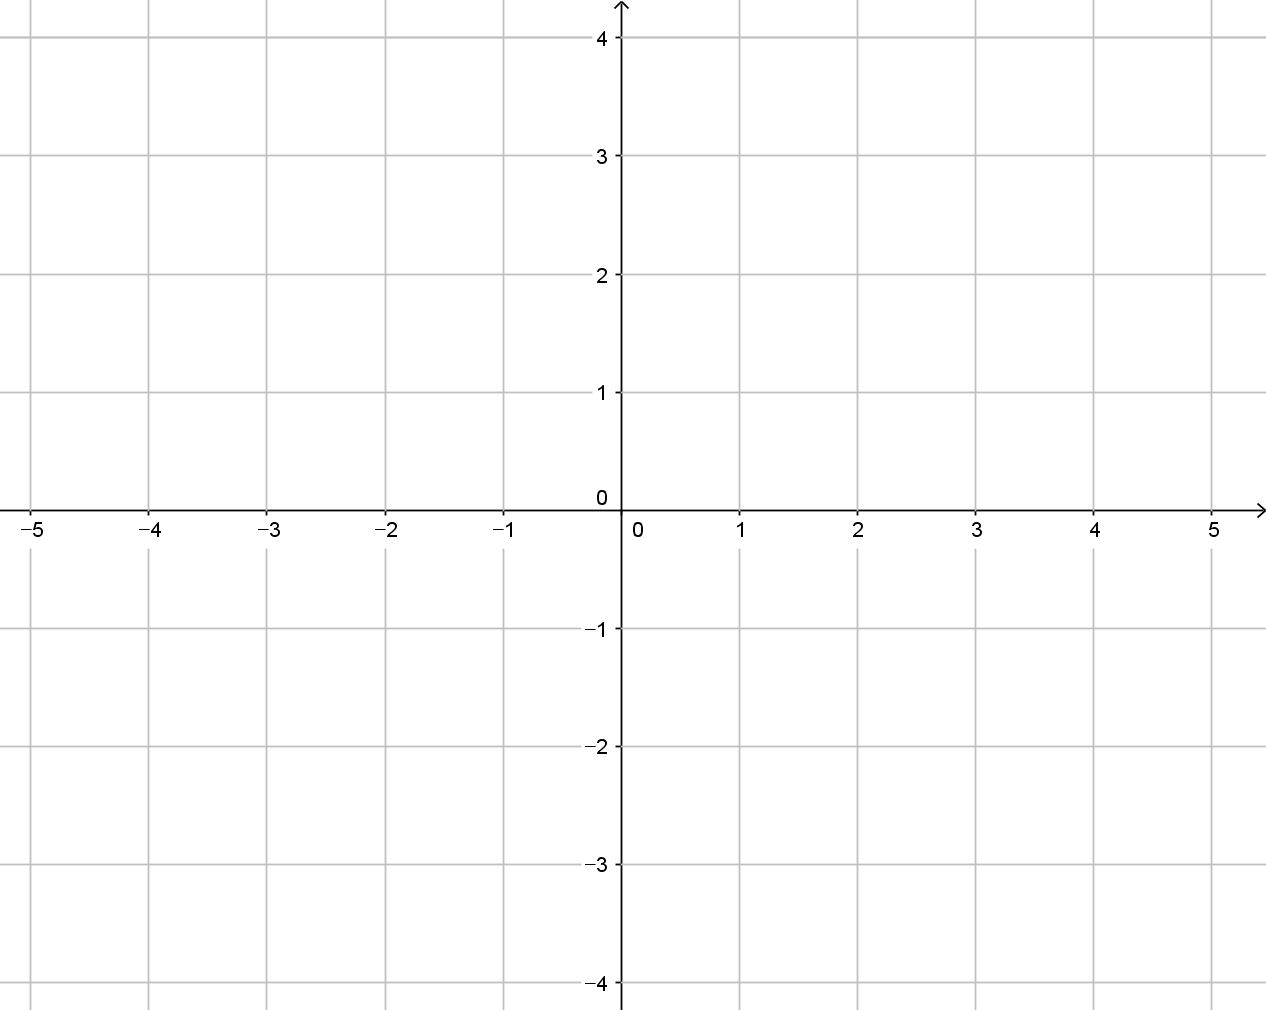
\includegraphics[width=0.5\textwidth]{5times4}
\end{figure*}
\[
\textbf{답 : }
\lim_{x\to-2-}g(x)=\pb1,\qquad
\lim_{x\to-2+}g(x)=\pb1,\qquad
\lim_{x\to-2}g(x)=\pb1.
\]
\clearpage
%
\item
\(h(x)=|x-3|-2\)
\tabto{0.5\textwidth}\(\langle x=3\rangle\)
\begin{figure*}[h!]
\centering
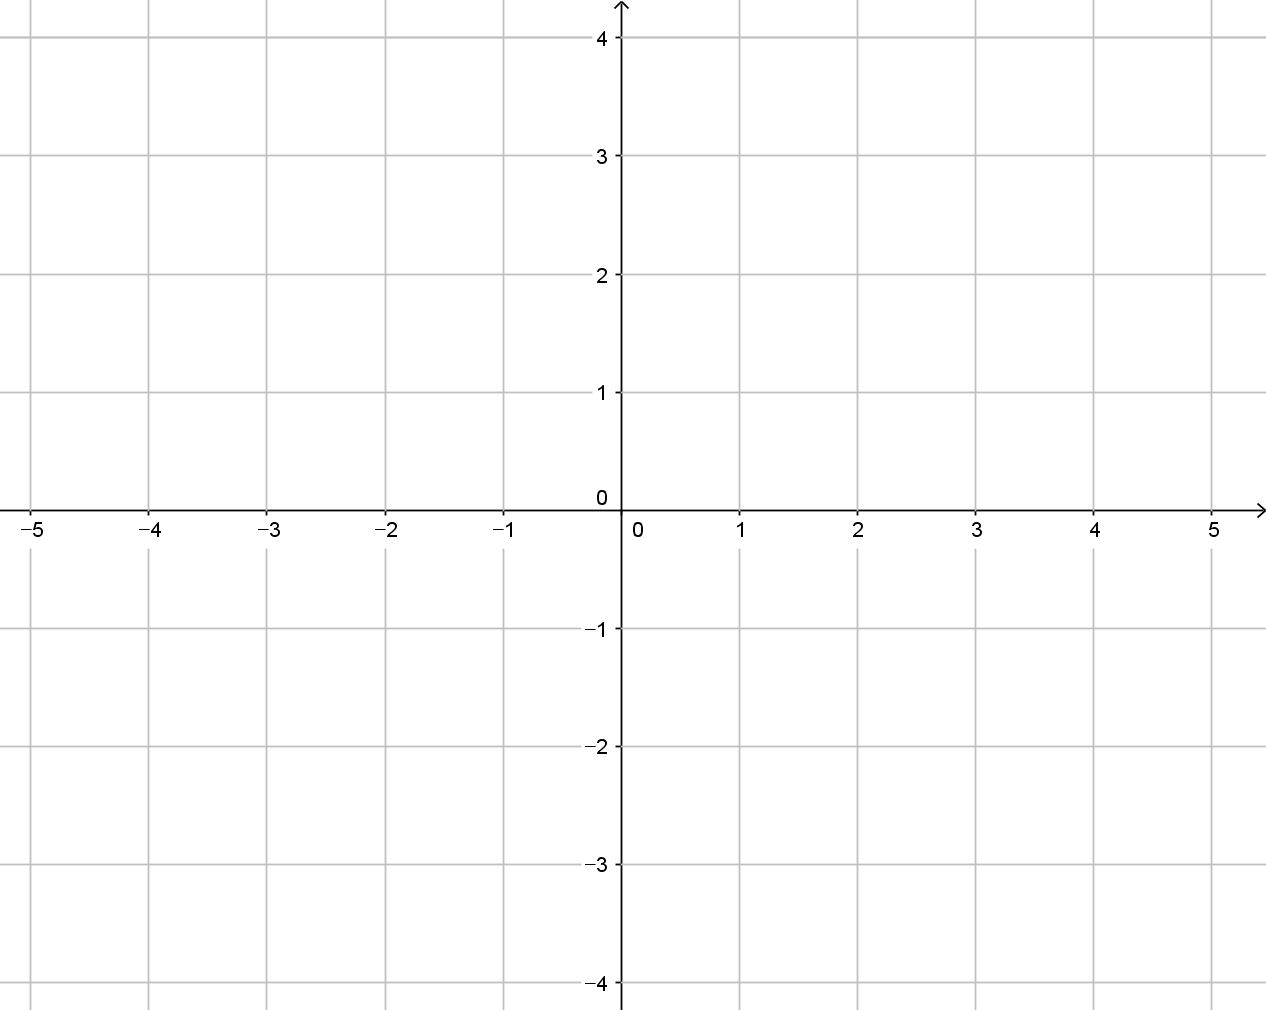
\includegraphics[width=0.5\textwidth]{5times4}
\end{figure*}
\[
\textbf{답 : }
\lim_{x\to3-}h(x)=\pb1,\qquad
\lim_{x\to3+}h(x)=\pb1,\qquad
\lim_{x\to3}h(x)=\pb1.
\]
%
\item
\(k(x)=[x]\)
\tabto{0.5\textwidth}\(\langle x=0\rangle\)\\
(단, \([x]\)는 \(x\)보다 크지 않은 최대 정수)
\begin{figure*}[h!]
\centering
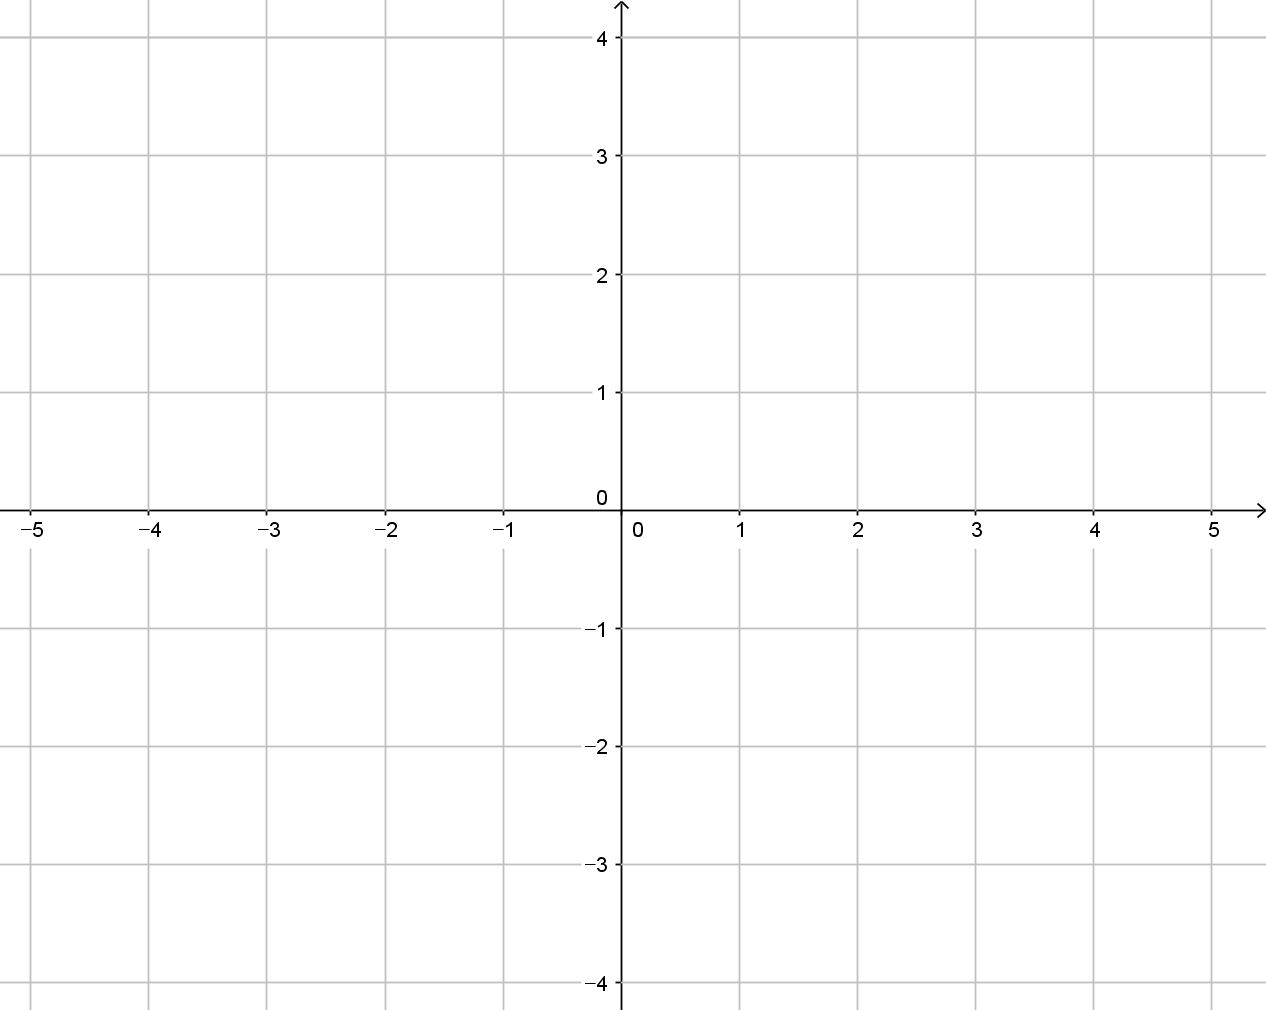
\includegraphics[width=0.5\textwidth]{5times4}
\end{figure*}\[
\textbf{답 : }
\lim_{x\to0-}k(x)=\pb1,\qquad
\lim_{x\to0+}k(x)=\pb1,\qquad
\lim_{x\to0}k(x)=\pb1.
\]
\end{enumerate}

%%
\section{함수의 극한에 대한 성질}
\begin{mdframed}[innertopmargin=-5pt]
%
\theo{함수의 극한에 대한 성질}\label{basic_property}
\(\displaystyle\lim_{x\to a}f(x)\)와 \(\displaystyle\lim_{x\to a}g(x)\)가 모두 존재할 때, 다음이 성립한다.

\bigskip
\begin{enumerate}[label=(\(\alph*\))]
\item
\(\displaystyle\lim_{x\to a}kf(x)=k\lim_{x\to a}f(x)\)
\item
\(\displaystyle\lim_{x\to a}\left(f(x)+g(x)\right)=\lim_{x\to a}f(x)+\lim_{x\to a}g(x)\)
\item
\(\displaystyle\lim_{x\to a}\left(f(x)-g(x)\right)=\lim_{x\to a}f(x)-\lim_{x\to a}g(x)\)
\item
\(\displaystyle\lim_{x\to a}f(x)g(x)=\lim_{x\to a}f(x)\lim_{x\to a}g(x)\)
\item
\(\displaystyle\lim_{x\to a}\frac{f(x)}{g(x)}
=\frac{\displaystyle\lim_{x\to a}f(x)}{\displaystyle\lim_{x\to a}g(x)}\)
\end{enumerate}
\end{mdframed}
위의 성질은 \(x\to a\)를 \(x\to a+\), \(x\to a-\), \(x\to\infty\), \(x\to-\infty\)로 바꾸어도 여전히 성립한다.

%
\exam{}
\begin{enumerate}
\item
\(\displaystyle\lim_{x\to2}(x^2-2x)=\lim_{x\to2}x^2-\lim_{x\to2}2x
=\lim_{x\to2}x^2-2\lim_{x\to2}x=4-2\times2=0\)
\item
\(\displaystyle\lim_{x\to2+}\left([x]+|x-2|\right)=\lim_{x\to2+}[x]+\lim_{x\to2+}|x-2|=2+0=2\)
\item
\(\displaystyle\lim_{x\to\infty}\left(\frac1x+2\right)\left(-\frac3x+1\right)
=\lim_{x\to\infty}\left(\frac1x+2\right)\lim_{x\to\infty}\left(-\frac3x+1\right)
=2\times1=2\)
\item
\(\displaystyle\lim_{x\to2}\frac{x^2}{x+2}
=\frac{\displaystyle\lim_{x\to2}x^2}{\displaystyle\lim_{x\to2}x+2}=\frac44=1\)
\end{enumerate}

\clearpage
%
\prob{}
%정리 \ref{basic_property}를 사용하여
다음 극한값들을 계산하시오.
\begin{enumerate}
\item
\(\displaystyle\lim_{x\to\infty}\left(\frac1{x^2}+\frac{2x+1}x\right)\)
\item
\(\displaystyle\lim_{x\to1-}(x-[x])\)
\item
\(\displaystyle\lim_{x\to4}3x\sqrt{x}\)
\item
\(\displaystyle\lim_{x\to0}\frac{x^2+4x+3}{x+1}\)
\end{enumerate}

%
\prob{}
\(\displaystyle\lim_{x\to a}f(x)=2\)와 \(\displaystyle\lim_{x\to a}g(x)=-5\)일 때, 다음 값들을 계산하시오.
\begin{enumerate}
\item
\(\displaystyle\lim_{x\to a}5f(x)\)
\item
\(\displaystyle\lim_{x\to a}\left\{3+2g(x)\right\}\)
\item
\(\displaystyle\lim_{x\to a}\left\{f(x)+g(x)\right\}\)
\item
\(\displaystyle\lim_{x\to a}\left\{3f(x)+4g(x)\right\}\)
\end{enumerate}

%%
\section{함수의 극한값과 대소관계}
두 함수 \(f(x)\), \(g(x)\)에 대하여
\begin{mdframed}
\[f(x)\le g(x)\quad\Longrightarrow\quad\lim_{x\to a}f(x)\le\lim_{x\to a}g(x)\]
\end{mdframed}
가 성립한다.
하지만,
\begin{mdframed}
\[f(x)<g(x)\quad\Longrightarrow\quad\lim_{x\to a}f(x)<\lim_{x\to a}g(x)\]
\end{mdframed}
가 성립하지는 않는다.

\kswrapfig[Pos=r,Width=3cm]{sandwich}{
예를 들어,
\[f(x)=2x-1,\qquad g(x)=\begin{cases}x^2&(x\neq1)\\2&(x=1)\end{cases}\]
이면 \(f(x)<g(x)\)이지만,
\[\lim_{x\to 1}f(x)=\lim_{x\to 1}g(x)\]
이다.
}%\begin{figure*}[h!]
%\centering
%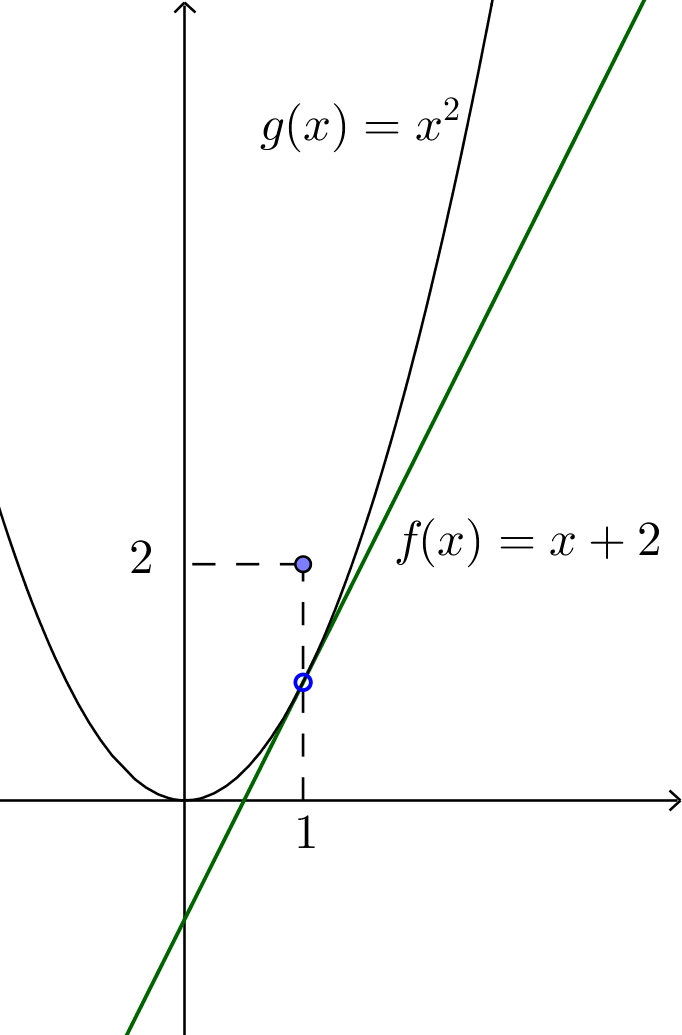
\includegraphics[width=0.4\textwidth]{sandwich}
%\end{figure*}

대신
\begin{mdframed}
\[f(x)<g(x)\quad\Longrightarrow\quad\lim_{x\to a}f(x)\le\lim_{x\to a}g(x)\]
\end{mdframed}
는 성립한다.
위의 성질도 마찬가지로 \(x\to a\)를 \(x\to a+\), \(x\to a-\), \(x\to\infty\), \(x\to-\infty\)로 바꾸어도 여전히 성립한다.

%
\exam{}
함수 \(f(x)\)가 \(x>0\)인 모든 실수 \(x\)에 대해
\[4-x\le f(x)\le\frac4x\]
을 만족시킬 때, \(\displaystyle\lim_{x\to2}f(x)\)를 구하여라.
\begin{mdframed}
\(4-x\le f(x)\le\frac4x\)이므로
\[\lim_{x\to 2}(4-x)\le\lim_{x\to 2}f(x)\le\lim_{x\to 2}\frac4x\]
\[2\le\lim_{x\to 2}f(x)\le2\]
따라서
\[\lim_{x\to 2}f(x)=2\]
\end{mdframed}

%
\prob{}
함수 \(f(x)\)가 \(x\neq1\), \(x\neq3\)인 모든 실수 \(x\)에 대해
\[\frac{3x-4}{x-3}<f(x)<\frac{6x+3}{2x-2}\]
을 만족시킬 때, \(\displaystyle\lim_{x\to\infty}f(x)\)를 구하여라.
\procedure{0.45}
\ans

%%
\section*{답}
\begin{minipage}{.49\textwidth}
%
\an{5}
(1) \(2\)\\
(2) \(2\)\\
(3) \(-3\)

%
\an{8}
\(1\), \(1\)

%
\an{10}
\(\infty\)

%
\an{12}
\(-\infty\), \(\infty\)

%
\an{13}
\(\infty\), \(\infty\)

%
\an{18}
\begin{enumerate}[itemsep=0pt,topsep=0pt]
\item
\(2\), \(2\), \(2\)
\item
\(-1\), \(2\), \(\times\)
\item
\(-2\), \(-2\), \(-2\)
\item
\(-1\), \(0\), \(\times\)
\end{enumerate}

\end{minipage}
\begin{minipage}{.49\textwidth}
%
\an{21}
\begin{enumerate}[itemsep=0pt,topsep=0pt]
\item
\(2\)
\item
\(1\)
\item
\(24\)
\item
\(3\)
\end{enumerate}

%
\an{22}
\begin{enumerate}[itemsep=0pt,topsep=0pt]
\item
\(10\)
\item
\(-7\)
\item
\(-3\)
\item
\(-14\)
\end{enumerate}

%
\an{24}
\(3\)
\end{minipage}

\end{document}